% Tikz tree styling
\tikzstyle{level 1}=[level distance=3.0cm, sibling distance=1.5cm]
\tikzstyle{level 2}=[level distance=3.0cm, sibling distance=1.25cm]
\tikzstyle{sty} = [text width=3em, text centered]

\section{Introduction}

Monadic streams present an interesting way of programming with effects. 

They encapsulate the notion of a stream of values, where traversing the stream from one element to the next can result in, for example, more than one element, or maybe no elements at all. Traversing the stream could also require extra inputs, or cause I/O events, such as printing to the screen or asking for user interaction. These extra computations, among others, come under the umbrella term \emph{computational effects} or simply \emph{effects}. 

We will also call these effects \emph{monadic actions} or just \emph{actions}, referring to monads; these encapsulate the concept of effectful computations. \\

To understand monadic streams, we must first look at pure streams.

A \emph{pure stream} is an infinite sequence of values, for example
\begin{haskell}
  nats = 0 <: 1 <: 2 <: 3 <: 4 <: (*...*)
\end{haskell}
The type of pure streams with elements of type \verb+a+ is denoted by \verb+Stream a+. The cons operation \verb+(<:)+ is used to append an element in front of an existing stream. Streams are infinite, so we must use recursion to define them.

For example, the constant stream of ones is defined as
\begin{haskell}
  ones = 1 <: ones
\end{haskell}

The list of natural numbers can be defined as
\begin{haskell}
  nats = fromNat 0
    where fromNat n = n <: fromNat (n+1)
\end{haskell}

This kind of recursion is called \emph{corecursion}, the distinction being that there is no base case. For this to work in practice, corecursive structures (like our stream of natural numbers above) must be evaluated \emph{lazily}, meaning 'only as needed'. The lazy evaluation strategy allows definitions like this in Haskell and other similar programming languages. \\
  
A \emph{monadic stream} (which we call a \emph{monster} for short) is a sequence of values in which every constructor \verb+(<:)+ is guarded by a monadic action: to obtain the head (first element) and tail (continuation) of the stream, we must execute the monadic action. \\

For example a \emph{Maybe-monster} is a sequence of elements that is either nothing (meaning the sequence is finished) or some head element followed by a tail. This allows us to define both finite and infinite sequences. The definitions of \verb+ones+ and \verb+nats+ are still valid Maybe-monsters. In addition, we can now define finite sequences:
\begin{haskell}
  1 <: 2 <: 3 <: empty
\end{haskell}
where \verb+empty+ is the Maybe-monster given by the 'nothing' action. 

Another example is \emph{List-monsters}, where the effect is to produce a list of values, which can be thought of as a non-deterministic computation. An element consists of a list of heads and tails: there may be many (zero or more) branches, each with its own head and tail.
List-monsters are actually arbitrarily branching trees:
\begin{haskell}
node [ 5 <: leaf
     , 9 <: node [ 1 <: leaf
                 ]
     , 2 <: node [ 4 <: node [ 3 <: leaf
                             , 6 <: leaf
                             ]
                 , 7 <: leaf
                 ]
     ]
\end{haskell}
\verb+leaf+ is a tree with no branches (\verb+leaf = node []+). This example is the List-monster that corresponds to the tree below. Each branch has its own tail, or collection of subtrees in this case. \\

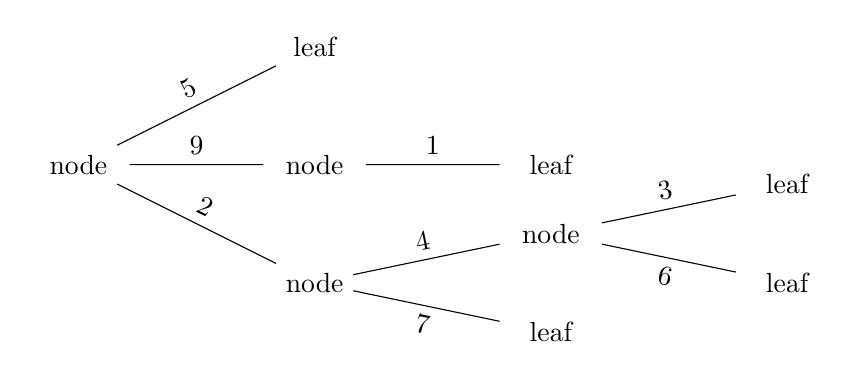
\begin{tikzpicture}[grow=right, sloped]
\node[sty] {node}
    child {
        node {node}
        child {
        		node[sty] {leaf}
        		edge from parent 
        		node[below] {$7$}
        }
	child {
        		node[sty] {node}
		child {
        			node[sty] {leaf}
        			edge from parent 
        			node[below] {$6$}
        		}
		child {
        			node[sty] {leaf}
        			edge from parent 
        			node[above] {$3$}
        		}
        		edge from parent 
        		node[above] {$4$}
        }
        edge from parent 
        node[above] {$2$}
    }
    child {
        node[sty] {node}
        child {
        		node[sty] {leaf}
        		edge from parent 
        		node[above] {$1$}
        }
        edge from parent 
        node[above] {$9$}
    }
    child {
        node[sty] {leaf}
        edge from parent 
        node[above] {$5$}
    };
\end{tikzpicture} \\

This is a finite tree, but the trees are allowed to be infinite, in both the width of the tree (the number of branches at one level), and the depth of the tree (the length of the longest path from the root to a leaf). \\

Some other types of monsters include \emph{IO-monsters}, which represent interactive processes, and \emph{Reader-monsters} which represent finite state automata. All of these variations of monadic stream we have introduced are explained and expanded on in section 4.

All of our examples will be written in Haskell, and sometimes pseudo-Haskell. In section 6, where we prove various properties of monsters, we will use Haskell for equational reasoning, alongside more type theoretic notation for the same purpose. These two notations are interwoven throughout the article, but the distinction between them should be clear: all Haskell code is surrounded with a black bounding box, and displayed in monospace font. \\

The primary purpose of this paper is to motivate the library we have developed: an extensive set of combinators and operations on monadic streams, along with some concrete examples, written in Haskell. This library is envisaged as motivation for the potential of monadic streams as a general model of intensional effectful computations. \\

To briefly explain the layout of the paper: the next two sections precisely define monadic streams, and the coindunction principle, the means by which we can prove properties of monadic streams (and, more generally, corecursive structures). 

Section 4 and 5 focus on developing concrete examples, and how specific functions from our library specialise in the different contexts presented by various kinds of monsters. 

In section 6 we begin to prove categorical properties of monadic streams. 

In the final two sections we talk about related work, specifically in Functional Reactive Programming (FRP), and conclude with open problems and general reflections.
